Odkrycie preferencji użytkownika ma na celu poznanie opinii na temat różnych 
usług i przedmiotów. Są one kluczem w wielu aplikacjach, takich jak systemy 
rekomendacji, filtrowanie lub wyszukiwanie informacji. W przypadku podejmowania 
decyzji poznanie preferencji jest jednym z podstawowych elementów systemu. Aby 
osiągnąć konsensus i przedstawić propozycje rozwiązań problemu, trzeba poznać 
zdanie decydentów na temat każdej z alternatyw. Okazuje się, że nie jest to 
łatwe zadanie, ponieważ każdy z ekspertów posiada swoje własne idee, cele, 
motywacje i osobowość. Prowadzi to do wniosku, że różne osoby mogą wyrażać 
swoje preferencje na różne sposoby.

W tym rozdziale zostanie przedstawiony ogólny model poznawania preferencji. 
Następnie wprowadzone zostaną klasyczne sposoby reprezentacji. Warto zwrócić 
uwagę na to, że przed metodami klasycznymi stoi kilka wyzwań. Jednym z nich 
jest niepewność. Na przykład opis alternatywy lub wprowadzone preferencje mogą 
być niepełne i nieprecyzyjne ze względu na brak pełnej informacji, niewiedzę 
lub niezdecydowanie osoby. Dlatego na koniec rozdziału omówione zostaną metody 
wykorzystujące zbiory rozmyte.


\section{Model ogólny}
Scenariusz idealny zakłada poproszenie użytkowników o wyrażenie swoich 
preferencji na temat różnych cech ocenianego problemu. W praktyce ma to jednak 
ograniczone zastosowanie, a także nie zawsze jest to możliwe. Obiecującym 
źródłem odkrywania preferencji mogą być komentarze użytkowników. Ogólny schemat 
odkrywania i przetwarzania preferencji przedstawiony jest na rysunku
\ref{fig:ogolny_model_preferencji}.

Schemat zaproponowany przez Zenebe et al. [8] składa się z czterech głównych 
elementów: wydobycie i prezentacja cech, odkrycie preferencji, reprezentacja 
preferencji, zastosowanie wydobytych informacji.

\begin{figure}[ht]
  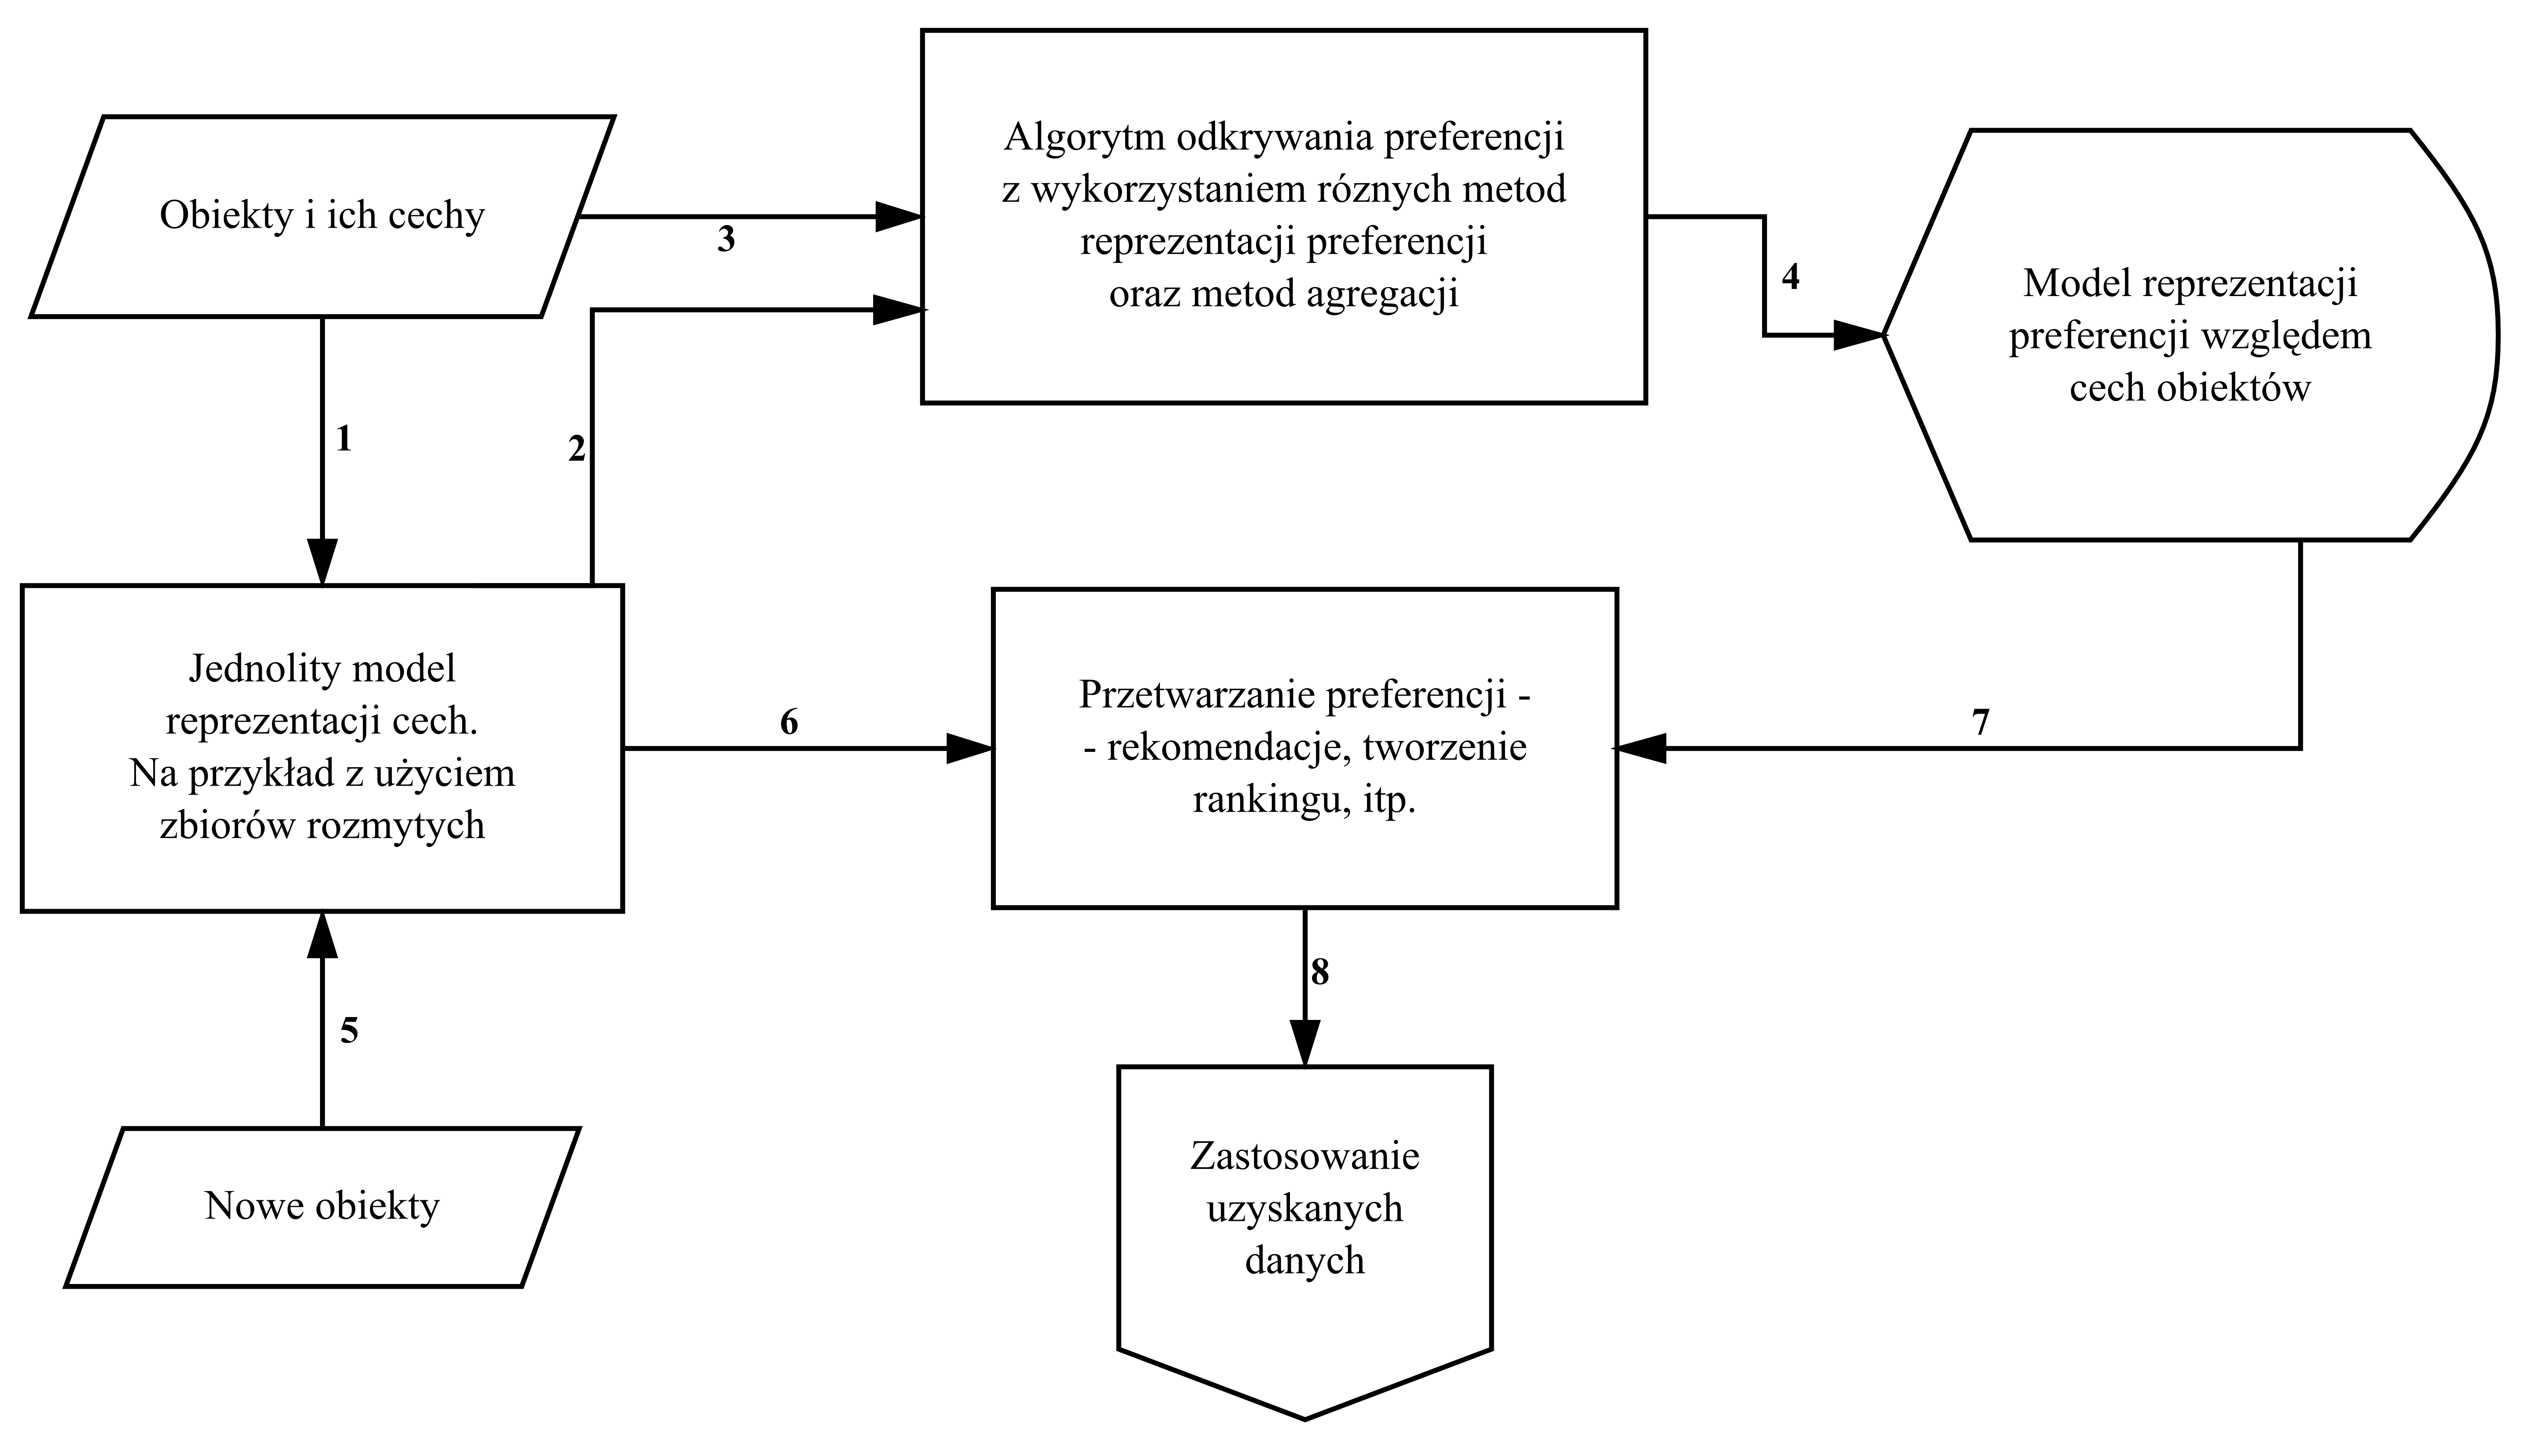
\includegraphics[width=\linewidth]
  	{chapters/preferences/ogolny_model_preferencji}
  \caption{Schemat odkrywania i przetwarzania preferencji}
  \label{fig:ogolny_model_preferencji}
\end{figure}

\section{Metody klasyczne}

\subsection{Uporządkowanie alternatyw}

W tym przypadku, alternatywy uporządkowane są od najlepszej do najgorszej bez
żadnej dodatkowej informacji. Formalnie, ekspert $e_k$ podaje swoje preferencje
dla zbioru alternatyw $\mathcal{X}$ jako indywidualne uporządkowanie alternatyw
$ O^k =$ $\{o^k(1), \dotsc,$ $o^k(n)\}$, gdzie $o^k(\cdot)$ jest funkcją
permutacji nad zbiorem indeksów $\{1,\dotsc,n\}$. Jak wspomniano wyżej, wynikiem
jest uporządkowany zbiór alternatyw.

\subsection{Multiplikatywna relacja preferencji}
W tym przypadku, preferencje ekspertów dla zbioru $\mathcal{X}$ opisane są przy
pomocy relacji preferencji $A^k \subset X \times X, A^k = a^k_{ij}$, gdzie
$a^k_{ij}$ wskazuje stopień intensywności preferencji alternatywy $x_i$ do
$x_j$. Innymi słowy, alternatywa $x_i$ jest $a^k_{ij}$ razy tak dobra jak $x_j$.

Nawiązując do pracy Millera \todo{bibl} nad postrzeganiem liczb, Saaty w swojej
pracy \todo{bibl} sugeruje używania w takich sytuacjach skali od $1$ do $9$.
Zatem $a^k_{ij} = 1$ interpretuje się jako obojętność lub brak różnicy dla
eksperta pomiędzy rozwiązaniami $x_i$ oraz $x_j$, $a^k_{ij}=9$ oznacza, że $x_i$
jest zdecydowanie bardziej preferowane niż $x_j$, natomiast $a^k_{ij} \in \{
2,3, \dotsc, 8\}$ oznacza oceny pośrednie. Z reguły zakłada się, że relacja jest
wzajemnie odwrotna, czyli $\forall_{i,j} \, a^k_{ij} \cdot a^k_{ji} = 1$.

\subsection{Funkcja użyteczności}
Użyteczność to inaczej zdolność dobra do zaspokajania potrzeb. Określa
subiektywną przyjemność, pożytek lub zadowolenie płynące z dokonanego wyboru.
Należy pamiętać, że użyteczność jest abstrakcją i ma charakter subiektywny,
podobnie jak pozostałe metody. Przy pomocy funkcji użyteczności, ekspert
przedstawia ocenę każdej z alternatyw zgodnie z użytecznością z jego punktu
widzenia. Formalnie, ekspert $e_k$ podaje swoje preferencje dla zbioru
alternatyw $\mathcal{X}$ jako zbiór $n$ wartości użyteczności $U^k = \{u^k_i;
i=1,\dotsc,n\}, u^k_i \in [0,1]$, gdzie $u^k_i$ reprezentuje wartość
użyteczności alternatywy $x_i$ daną przez eksperta $e_k$.

\section{Metody oparte na zbiorach rozmytych}
Teoria zbiorów rozmytych jest stosowana w grupowym podejmowaniu decyzji już od 
długiego czasu \todo{biblio}. Większość modeli opracowanych w literaturze jest 
opartych na rozmytej relacji preferencji, która może być uzyskana poprzez 
porównania pomiędzy parami różnych alternatyw przez ekspertów.

Z drugiej strony, wiele problemów dotyczy ilościowych aspektów, które mogą być 
ocenione przy użyciu konkretnych wartości liczbowych, czyli z użyciem opisanych 
wcześniej metod klasycznych. Jednakże, występuje bardzo dużo problemów o 
aspekcie jakościowym, które są bardzo trudne do oceny poprzez dokładne i ścisłe 
wartości. W takich przypadkach, podejście wykorzystujące zmienne lingwistyczne 
może być stosowane w celu uzyskania lepszego rozwiązania. Na przykład, gdy 
eksperci starają się ocenić komfort samochodu, gdzie są używane wyrażenia 
językowe, jak ,,dobry'', ,,niezły'', ,,słaby''.

\subsection{Rozmyta relacja preferencji}

\begin{definition}
Rozmyta relacja preferencji $R$ na zbiorze alternatyw $\mathcal{X}$ jest zbiorem
rozmytym na iloczynie kartezjańskim $X \times X$ z funkcją przynależności
$\mu_R : X \times X \rightarrow [0,1]$. Niech $P(x_i,x_j) \in R$ będzie rozmytą
relacją preferencji pomiędzy alternatywami $x_i$ i $x_j$. Wtedy $P(x_i,x_j)$
oraz $P(x_j,x_i)$ są zwrotne, tzn. $P(x_i,x_j) + P(x_j,x_i) = 1.$
\end{definition}

Niech $\mathcal{X}$ będzie zbiorem alternatyw oraz $x_i,x_j \in \mathcal{X}$.
Oznaczmy $P^k(x_i,x_j) = p^k_{ij}$, co oznacza stopień preferowania alternatywy 
$x_i$ nad $x_j$ względem kryterium $k$. Stąd $p^k_{ij} = 1$ oznacza, że
rozwiązanie $x_i$ jest bezwzględnie lepsze niż $x_j$, $p^k_{ij} \in (0.5; 1)$
przewagę $x_i$ nad $x_j$ (im większa wartość tym większa przewaga), a $x_j$,
$p^k_{ij} = 0.5$ brak różnicy pomiędzy rozwiązaniami.

Rozmyta relacja preferencji stosowana jest do modelowania
nieprecyzyjnej relacji pomiędzy różnymi rozwiązaniami. Aby zredukować uciążliwe
zadanie przypisywania stopni preferencji pomiędzy alternatywami przez ekspertów
($q(n-1)/2$ razy), rozmyta relacja preferencji między dwoma alternatywami $x_i$
i $x_j$ dla kryterium $k$ jest obliczana przez porównywanie parami ocen
lingwistycznych $g^t_k(x_i)$ i $g^t_k(x_j)$, które mogą być opisane jako liczby
rozmyte (szczegóły w następnym podpunkcie). W ten sposób, liczba ocen ekspertów
zmniejsza się do $qn$ razy.
\begin{figure}[ht]
  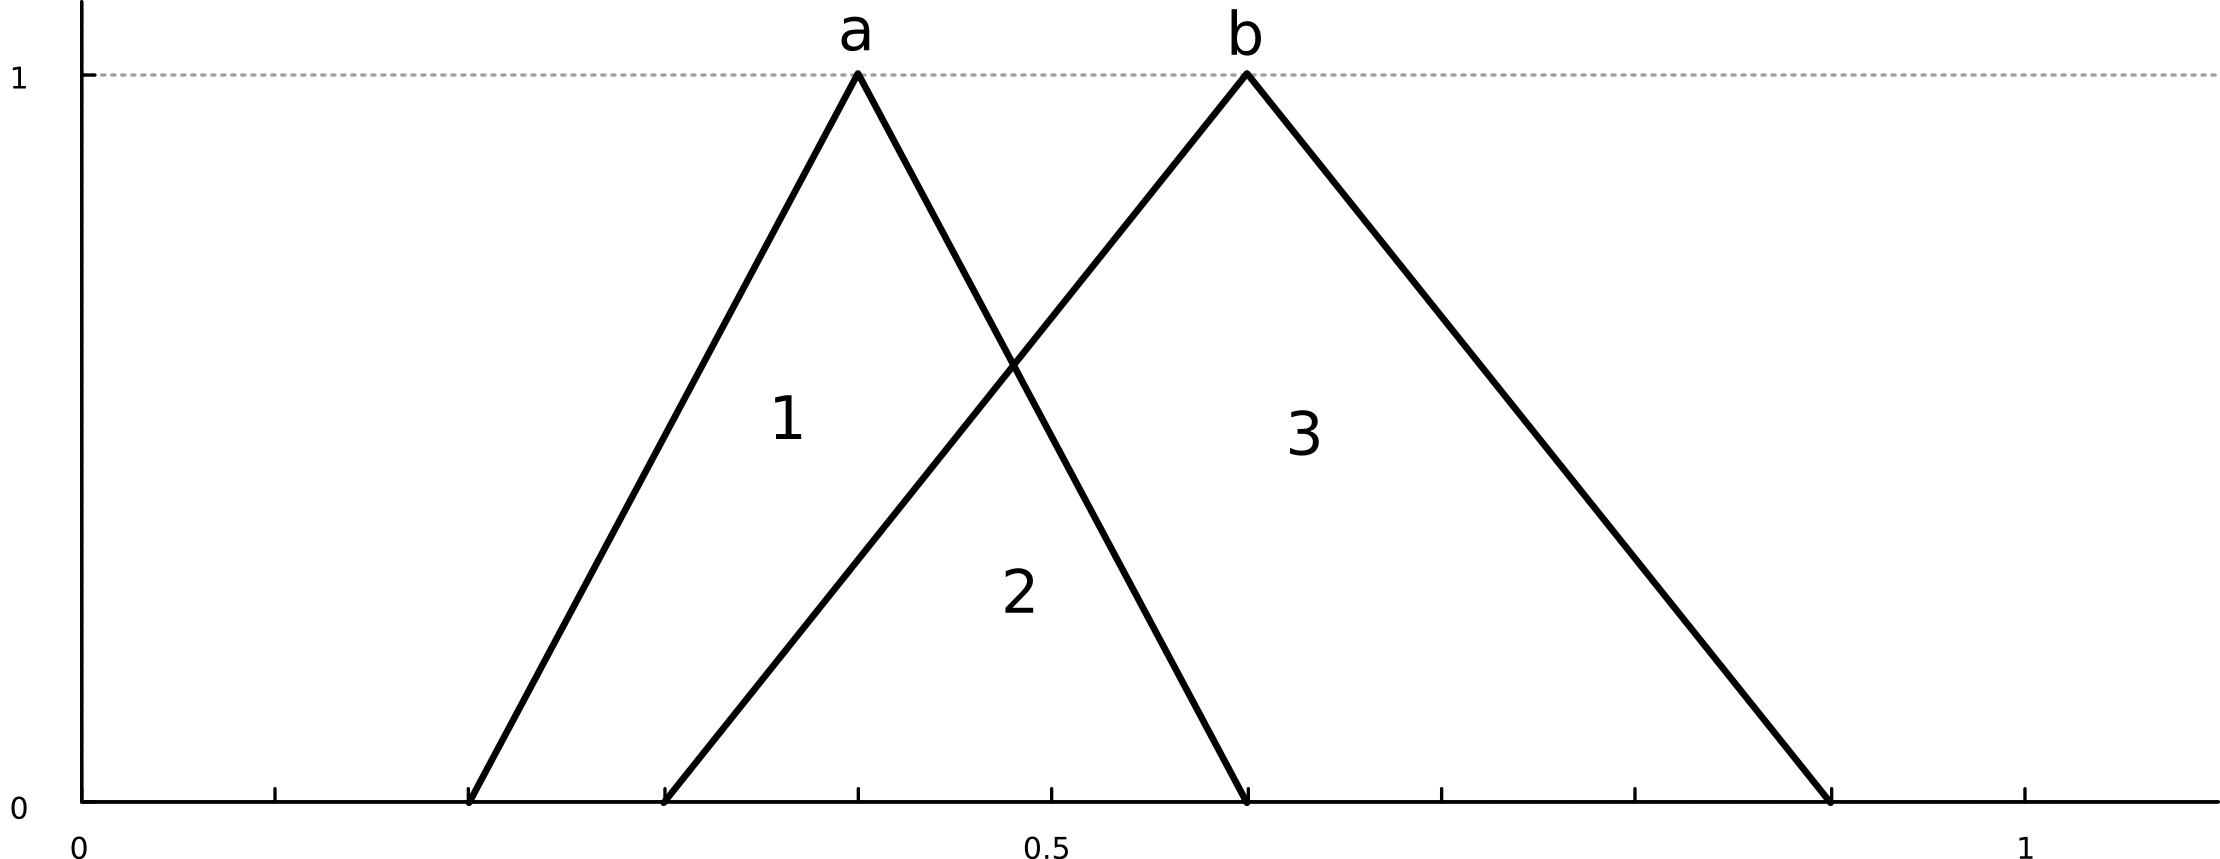
\includegraphics[width=\linewidth]
    {chapters/preferences/rozmyta_relacja_a}
  \caption{Przykład rozmytej relacji preferencji}
  \label{fig:rozmyta_relacja_preferencji}
\end{figure}
W literaturze istnieje wiele sposobów na zdefiniowanie relacji rozmytej pomiędzy
dwoma liczbami rozmytymi. W tej pracy zostanie użyte podejście Tsenga i Kleina
\todo{biblio} bazujące na odległości Hamminga ze względu na prostotę i
wydajność.

\begin{definition}
\label{def:rozmyta_relacja_preferencji}
Niech $a$ i $b$ będą liczbami rozmytymi. Rozmyte relacje preferencji $P(a,b)$ i
$P(b,a)$ zdefiniowane są w następujący sposób:
\begin{equation}
P(a,b) = \frac{D(a,b) + D(a \cap b, 0)}{D(a,0) + D(b,0)},
\end{equation}
\begin{equation}
P(b,a) = \frac{D(b,a) + D(a \cap b, 0)}{D(a,0) + D(b,0)},
\end{equation}
gdzie
\begin{itemize}
  \item[] $D(a,b)$ - powierzchnia, gdzie $a$ dominuje nad $b$,
  \item[] $D(b,a)$ - powierzchnia, gdzie $b$ dominuje nad $a$ (pole 1 i 3 na
  	rys. \ref{fig:rozmyta_relacja_preferencji}),
  \item[] $D(a,0)$ - powierzchnia $a$ (pole 1 i 2 na rys.
     \ref{fig:rozmyta_relacja_preferencji}),
  \item[] $D(b,0)$ - powierzchnia $b$ (pole 2 i 3 na rys.
  	\ref{fig:rozmyta_relacja_preferencji}),
  \item[] $D(a \cap b, 0)$ - przecięcie powierzchni $a$ i $b$ (pole 2 na rys.
  	\ref{fig:rozmyta_relacja_preferencji}).
\end{itemize}
\end{definition}

Dla przykładu rozmyta relacja preferencji na rysunku
\ref{fig:rozmyta_relacja_preferencji} jest liczona następująco:
$$P(a,b) = \frac{pole2}{(pole1 + pole2) + (pole2 + pole3)} = 0.18,$$
$$P(b,a) = \frac{(pole1 + pole3) + pole2}{(pole1 + pole2) + (pole2 + pole3)} =
0.82.$$

\subsection{Rozmyta relacja preferencji w przypadku wielu kryteriów}
Wyżej opisana rozmyta relacja preferencji pozwala ocenić alternatywy według
tylko jednego kryterium. W wielu przypadkach może się to okazać wystarczające,
ponieważ eksperci nie muszą oceniać poszczególnych cech rozwiązań, ale mogą
głosować bezpośrednio na nie po przeprowadzeniu dyskusji. Sytuacja komplikuje
się, kiedy każdy ekspert ocenia wyszczególnione wcześniej cechy rozwiązań (na
przykład cena, wygoda, wykonanie samochodu). W wyniku otrzymywany jest zbiór
relacji - po jednej na parę ekspert-kryterium. Aby uzyskać dane pozwalające na
uporządkowanie alternatyw należy połączyć wszystkie wyniki każdego eksperta
osobno.

Niech $p^t_k(x_i,x_j)$ będzie rozmytą relacją preferencji pomiędzy alternatywami
$x_i$ i $x_j$ dla kryterium $c_k$ oraz eksperta $e^t$ liczoną według definicji
\ref{def:rozmyta_relacja_preferencji}:
$$p^t_k(x_i,x_j) = P(g^t_k(x_i),g^t_k(x_j)).$$

Zbiorcza rozmyta relacja preferencji pomiędzy alternatywami $x_i$ i $x_j$ dla
eksperta $e^t$ może być uzyskana jako ważona suma wartości $p^t_k(x_i,x_j)$ po
wszystkich kryteriach $p^t(x_i,x_j) = \sum_{k=1}^{q} w_k \times p^t_k(x_i,x_j)$,
gdzie $\sum_{k=1}^{q} w_k = 1$.

Ostatecznie możliwe jest uporządkowanie alternatyw w częściowym porządku poprzez
wyliczenie stopnia dominacji każdej z alternatyw, czyli jak bardzo ekspert
$e^t$ wspiera dane rozwiązanie $x_i$. Oblicza się to jako średnia z
$p^t(x_i,x_j) \text{ dla } x_j \in \mathcal{X} \text{ i } x_j \neq x_i \colon
h^t(x_i) = \frac{1}{n-1} \sum_{x_j \in \mathcal{X}, x_j \neq x_i} p^t(x_i,x_j).$

\subsection{Ocena lingwistyczna}
Rozmyte podejście lingwistyczne używa zmiennych lingwistycznych, które
uczestniczą w procesie oceniania przy pomocy terminologii językowej zamiast
wartości liczbowych. Takie podejście jest odpowiednie dla wielu problemów,
ponieważ umożliwia przedstawienie indywidualnych preferencji w bardziej
bezpośredniej i odpowiedniej formie wtedy, gdy nie jest możliwe wyrażenie ich
precyzyjnie.

Zmienne lingwistyczne różnią się od numerycznych tym, że ich wartości nie są
liczbami, ale słowami lub zdaniami w naturalnym lub sztucznym języku. Ponieważ
słowa, generalnie, są mniej precyzyjne niż liczby, koncepcja zmiennych
lingwistycznych zapewnia środki umożliwiające zbliżoną charakteryzację zjawisk,
które są zbyt skomplikowane lub za słabo zdefiniowane, żeby opisać je w
tradycyjnych kategoriach ilościowych.
\begin{figure}[ht]
  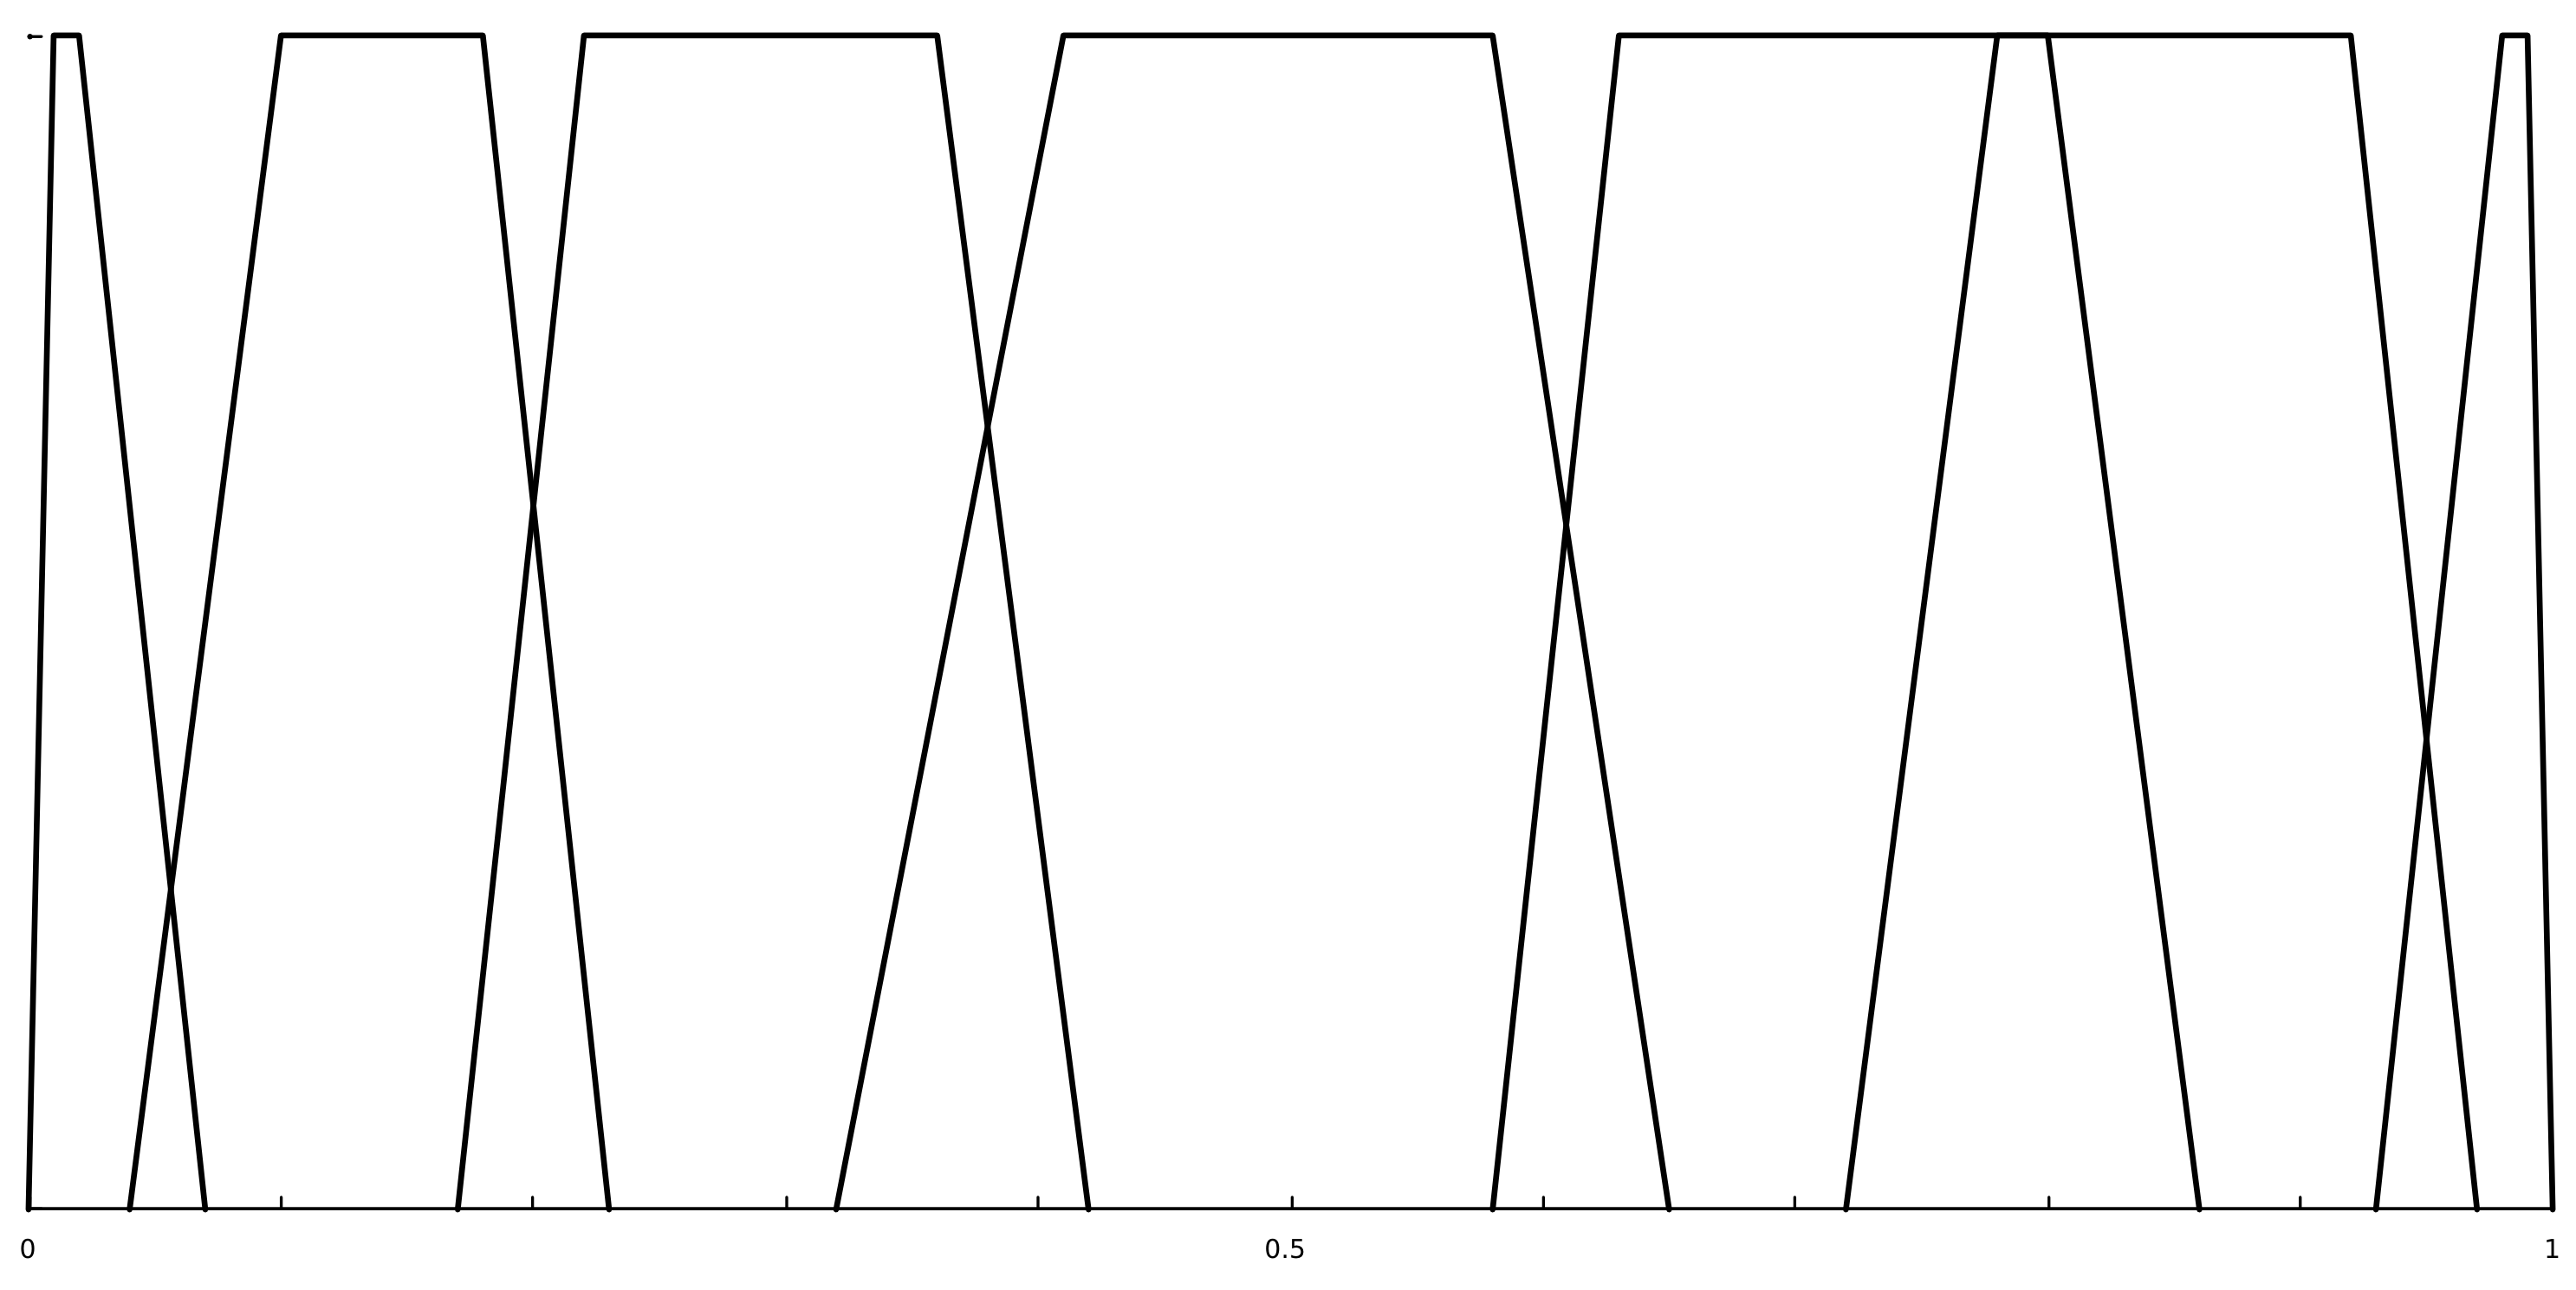
\includegraphics[width=\linewidth]
    {chapters/preferences/zbior_termow}
  \caption{Rozkład dziewięciu termów lingwistycznych}
  \label{fig:rozklad_dziewieciu_termow_lingwistycznych}
\end{figure}
Ze względu na to, że oceny lingwistyczne są przybliżonymi wartościami podanymi
przed decydentów, można uznać, że trapezowe funkcje przynależności są
wystarczające dobre, aby uchwycić niepewność oceny w procesie decyzyjnym.
Potrzebny jest również zbiór termów definiujący granularność niepewności. W
literaturze proponuje się zbiory o nieparzystej liczbie elementów rozłożonych
symetrycznie. Okazuje się również, że granularność, czyli moc zbioru, nie
powinna przekraczać 11 elementów. Dzięki temu unika się uzyskania zbyt
dokładnych wyników, co może być niemożliwe lub niepotrzebne. Co więcej, wybrany
zbiór powinien spełniać następujące warunki:
\begin{enumerate}[1)]
  \item uporządkowanie,
  \item operator negacji,
  \item operator maksimum,
  \item operator minimum.
\end{enumerate}

Przykładem może być następujący zbiór termów lingwistycznych przedstawiony
graficznie na rysunku \ref{fig:rozklad_dziewieciu_termow_lingwistycznych}
(pierwsze dwa parametry oznaczają przedział w którym wartość funkcji
przynależności jest 1, natomiast trzeci i czwarty parametr oznaczają lewą i
prawą szerokość rozkładu):

\begin{tabular}{lll}
P 	&	Pewne				 &	$(1, 1, 0, 0)$ \\
BM 	&	Bardzo Możliwe	 	 &	$(0.98, 0.99, 0.05, 0.01)$ \\
M 	&	Możliwe 			 &	$(0.78, 0.92, 0.06, 0.05)$ \\
ZS 	&	Znacząca Szansa 	 &	$(0.63,0.80,0.05,0.06)$ \\
MB 	&	Może Być 			 &	$(0.41, 0.58, 0.09, 0.07)$ \\
MS 	&	Mała Szansa			 &	$(0.22, 0.36, 0.05, 0.06)$ \\
BMS &	Bardzo Mała Szansa 	 &	$(0.1,0.18, 0.06, 0.05)$ \\
BMM &	Bardzo Mało Możliwe	 &	$(0.01, 0.02, 0.01,0.05)$ \\
N 	&	Niemożliwe 			 &	$(0, 0, 0, 0)$
\end{tabular}

\begin{figure}[ht]
  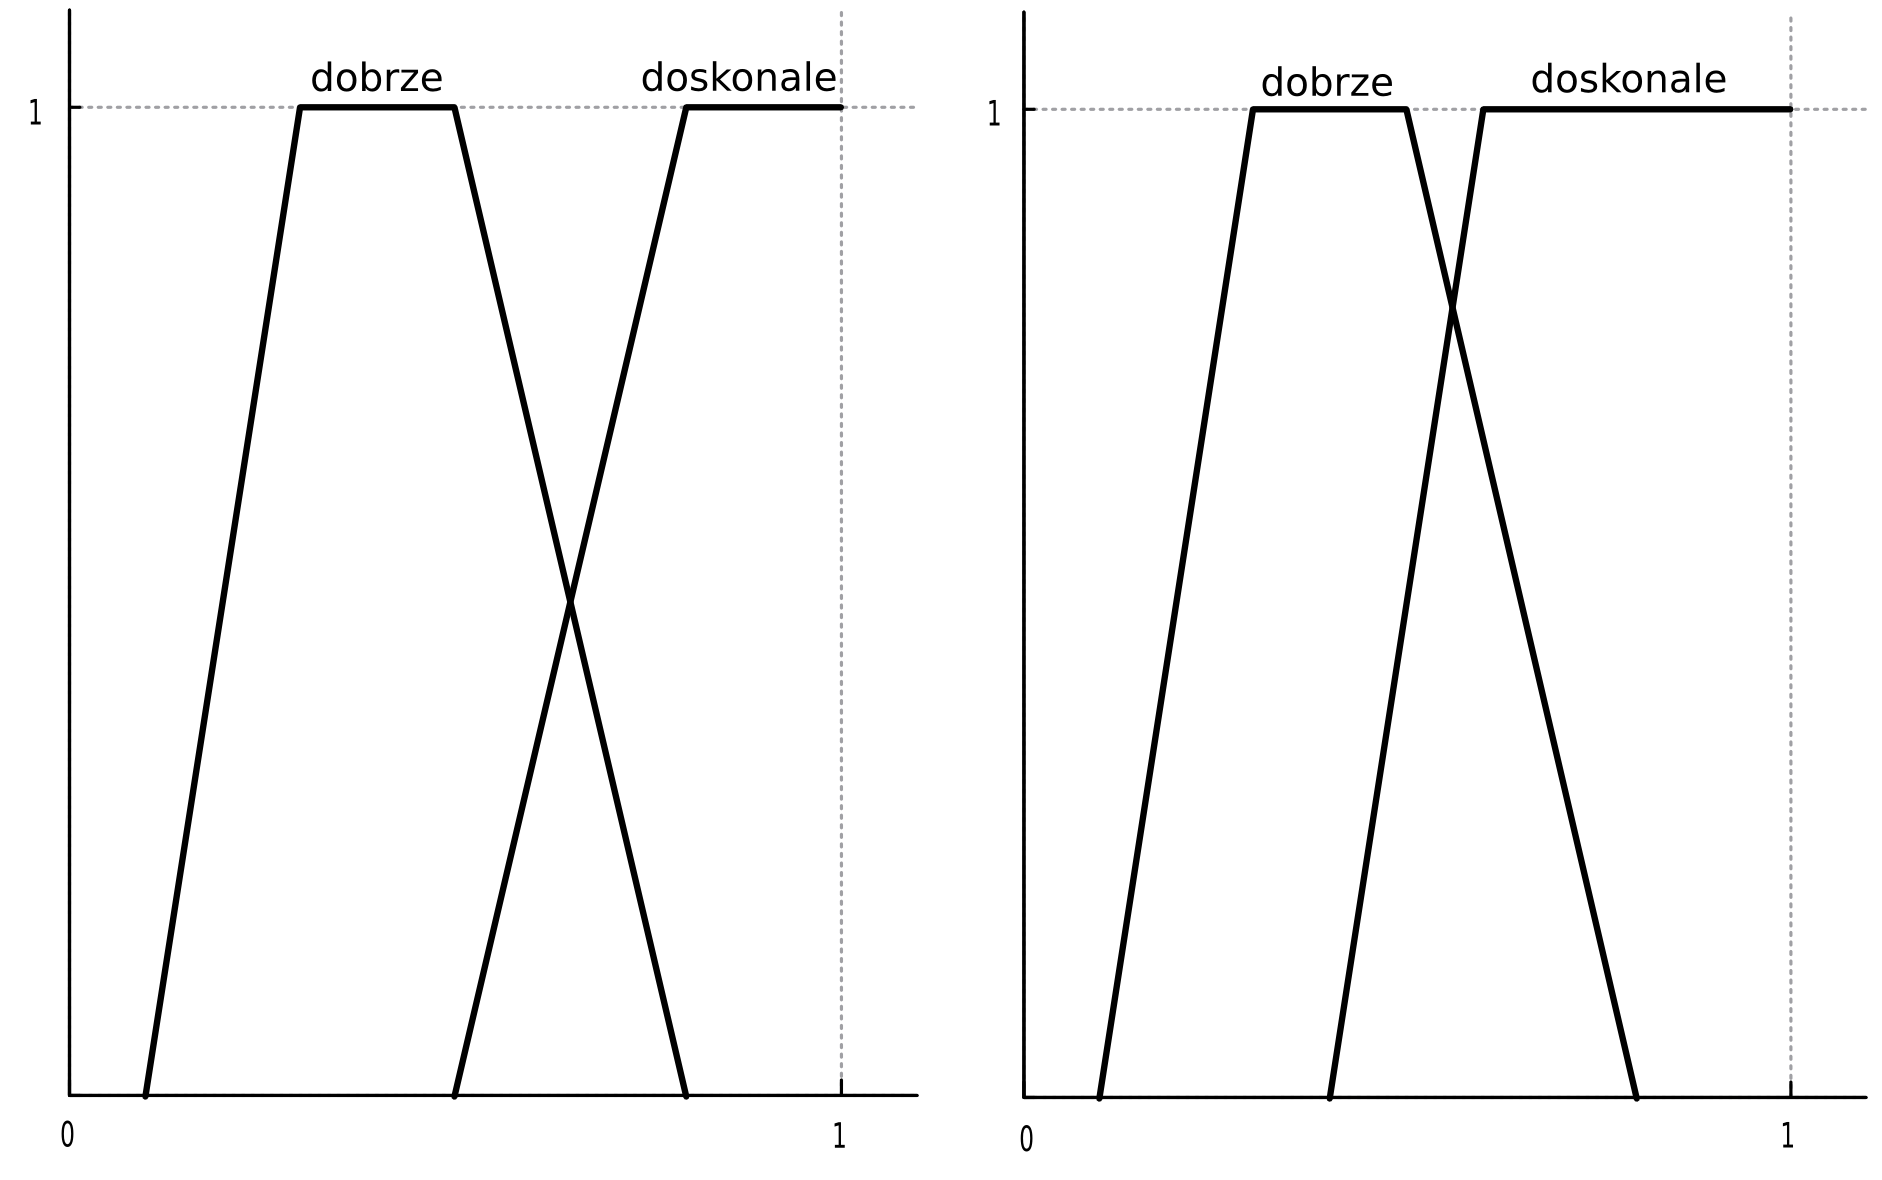
\includegraphics[width=\linewidth]
    {chapters/preferences/rozklad_podobnych_zmiennych}
  \caption{Podobne zmienne lingwistyczne}
  \label{fig:podobne_zmienne_lingwistyczne}
\end{figure}
Okazuje się, że nie można założyć, że wszyscy zgadzają się na takie same funkcje
przynależności przypisane do termów i nie ma jednego uniwersalnego rozkładu. Dla
przykładu można rozważyć dwie bardzo podobne koncepcje przedstawione na rysunku
\ref{fig:podobne_zmienne_lingwistyczne}, które z matematycznego punktu
widzenia bardzo się różnią. Powszechnie przyjmuje się i akceptuje, że
dostrojenie funkcji przynależności jest jednym z ważniejszych elementów w
kontroli procesu. Dobrze jest dostarczyć mechanizm pozwalający ekspertom na
takie dostrojenie, jednak na potrzeby tej pracy przyjmuje się środowisko, w
którym eksperci zgadzają się na odgórnie narzucony zestaw termów lingwistycznych
ze względu na to, że zmienna lingwistyczna ma służyć zapewnieniu środków
umożliwiających zbliżoną charakterystykę nieprecyzyjnej oceny preferencji.

\subsection{Niesymetryczna zmienna lingwistyczna}
Wiele problemów można oceniać przy pomocy opisanych wcześniej zmiennych
lingwistycznych, których termy są równomiernie i symetrycznie rozłożone.
Istnieją jednak problemy, które muszą korzystać ze zmiennych lingwistycznych,
które nie mają takich właściwości, to znaczy mają nierównomiernie i
niesymetrycznie rozłożony zbiór termów. Tego typu zmienne lingwistyczne nazywane
są niesymetrycznymi zmiennymi lingwistycznymi (rysunek
\ref{fig:niesymetryczna_zmienna}).
\begin{figure}[ht]
  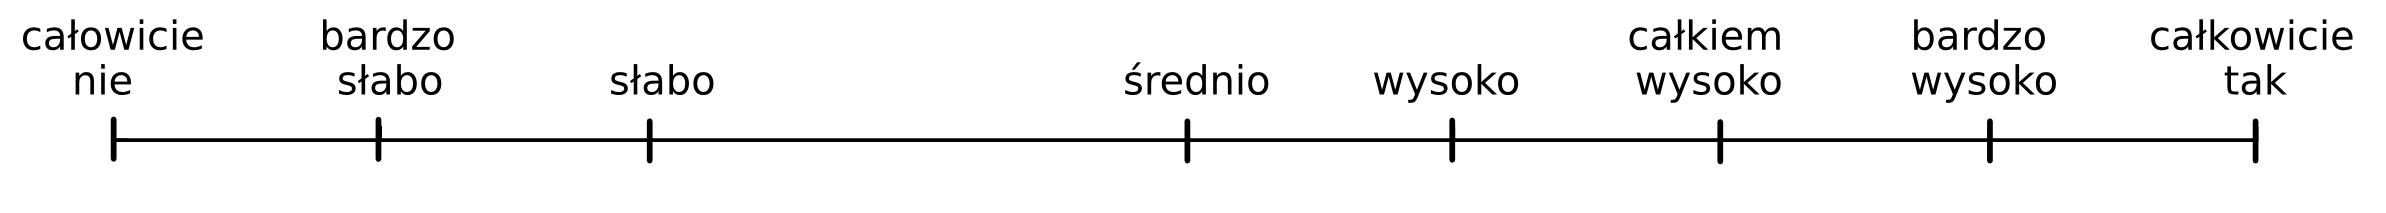
\includegraphics[width=\linewidth]
    {chapters/preferences/niesymetryczna_zmienna}
  \caption{Niesymetryczny rozkład termów}
  \label{fig:niesymetryczna_zmienna}
\end{figure}

W pracy dotyczącej informacji niesymetrycznej, Alonso et al. zaproponowali nowy
model radzenia sobie z niesymetrycznymi zmiennymi lingwistycznymi w procesie
podejmowania decyzji. W tym celu wykorzystana została tak zwana hierarchia
lingwistyczna, czyli zbiór poziomów, gdzie każdy poziom reprezentuje zbiór
termów lingwistycznych o odpowiedniej granularności. Każdy poziom oznaczany jest
jako $l(t, n(t))$, gdzie $t$ to numer porządkowy poziomu, a $n(t)$ to liczba
termów na poziomie $t$. Przez $S^{n(t)} = \{s^{n(t)}_0, \dotsc,
s^{n(t)}_{n(t)-1}\}$ oznacza się zbiór termów lingwistycznych na poziomie $t$.
Graficzny przykład hierarchii lingwistycznej pokazano na rysunku
\ref{fig:hierarchia_lingwistyczna}.
\begin{figure}[hb]
  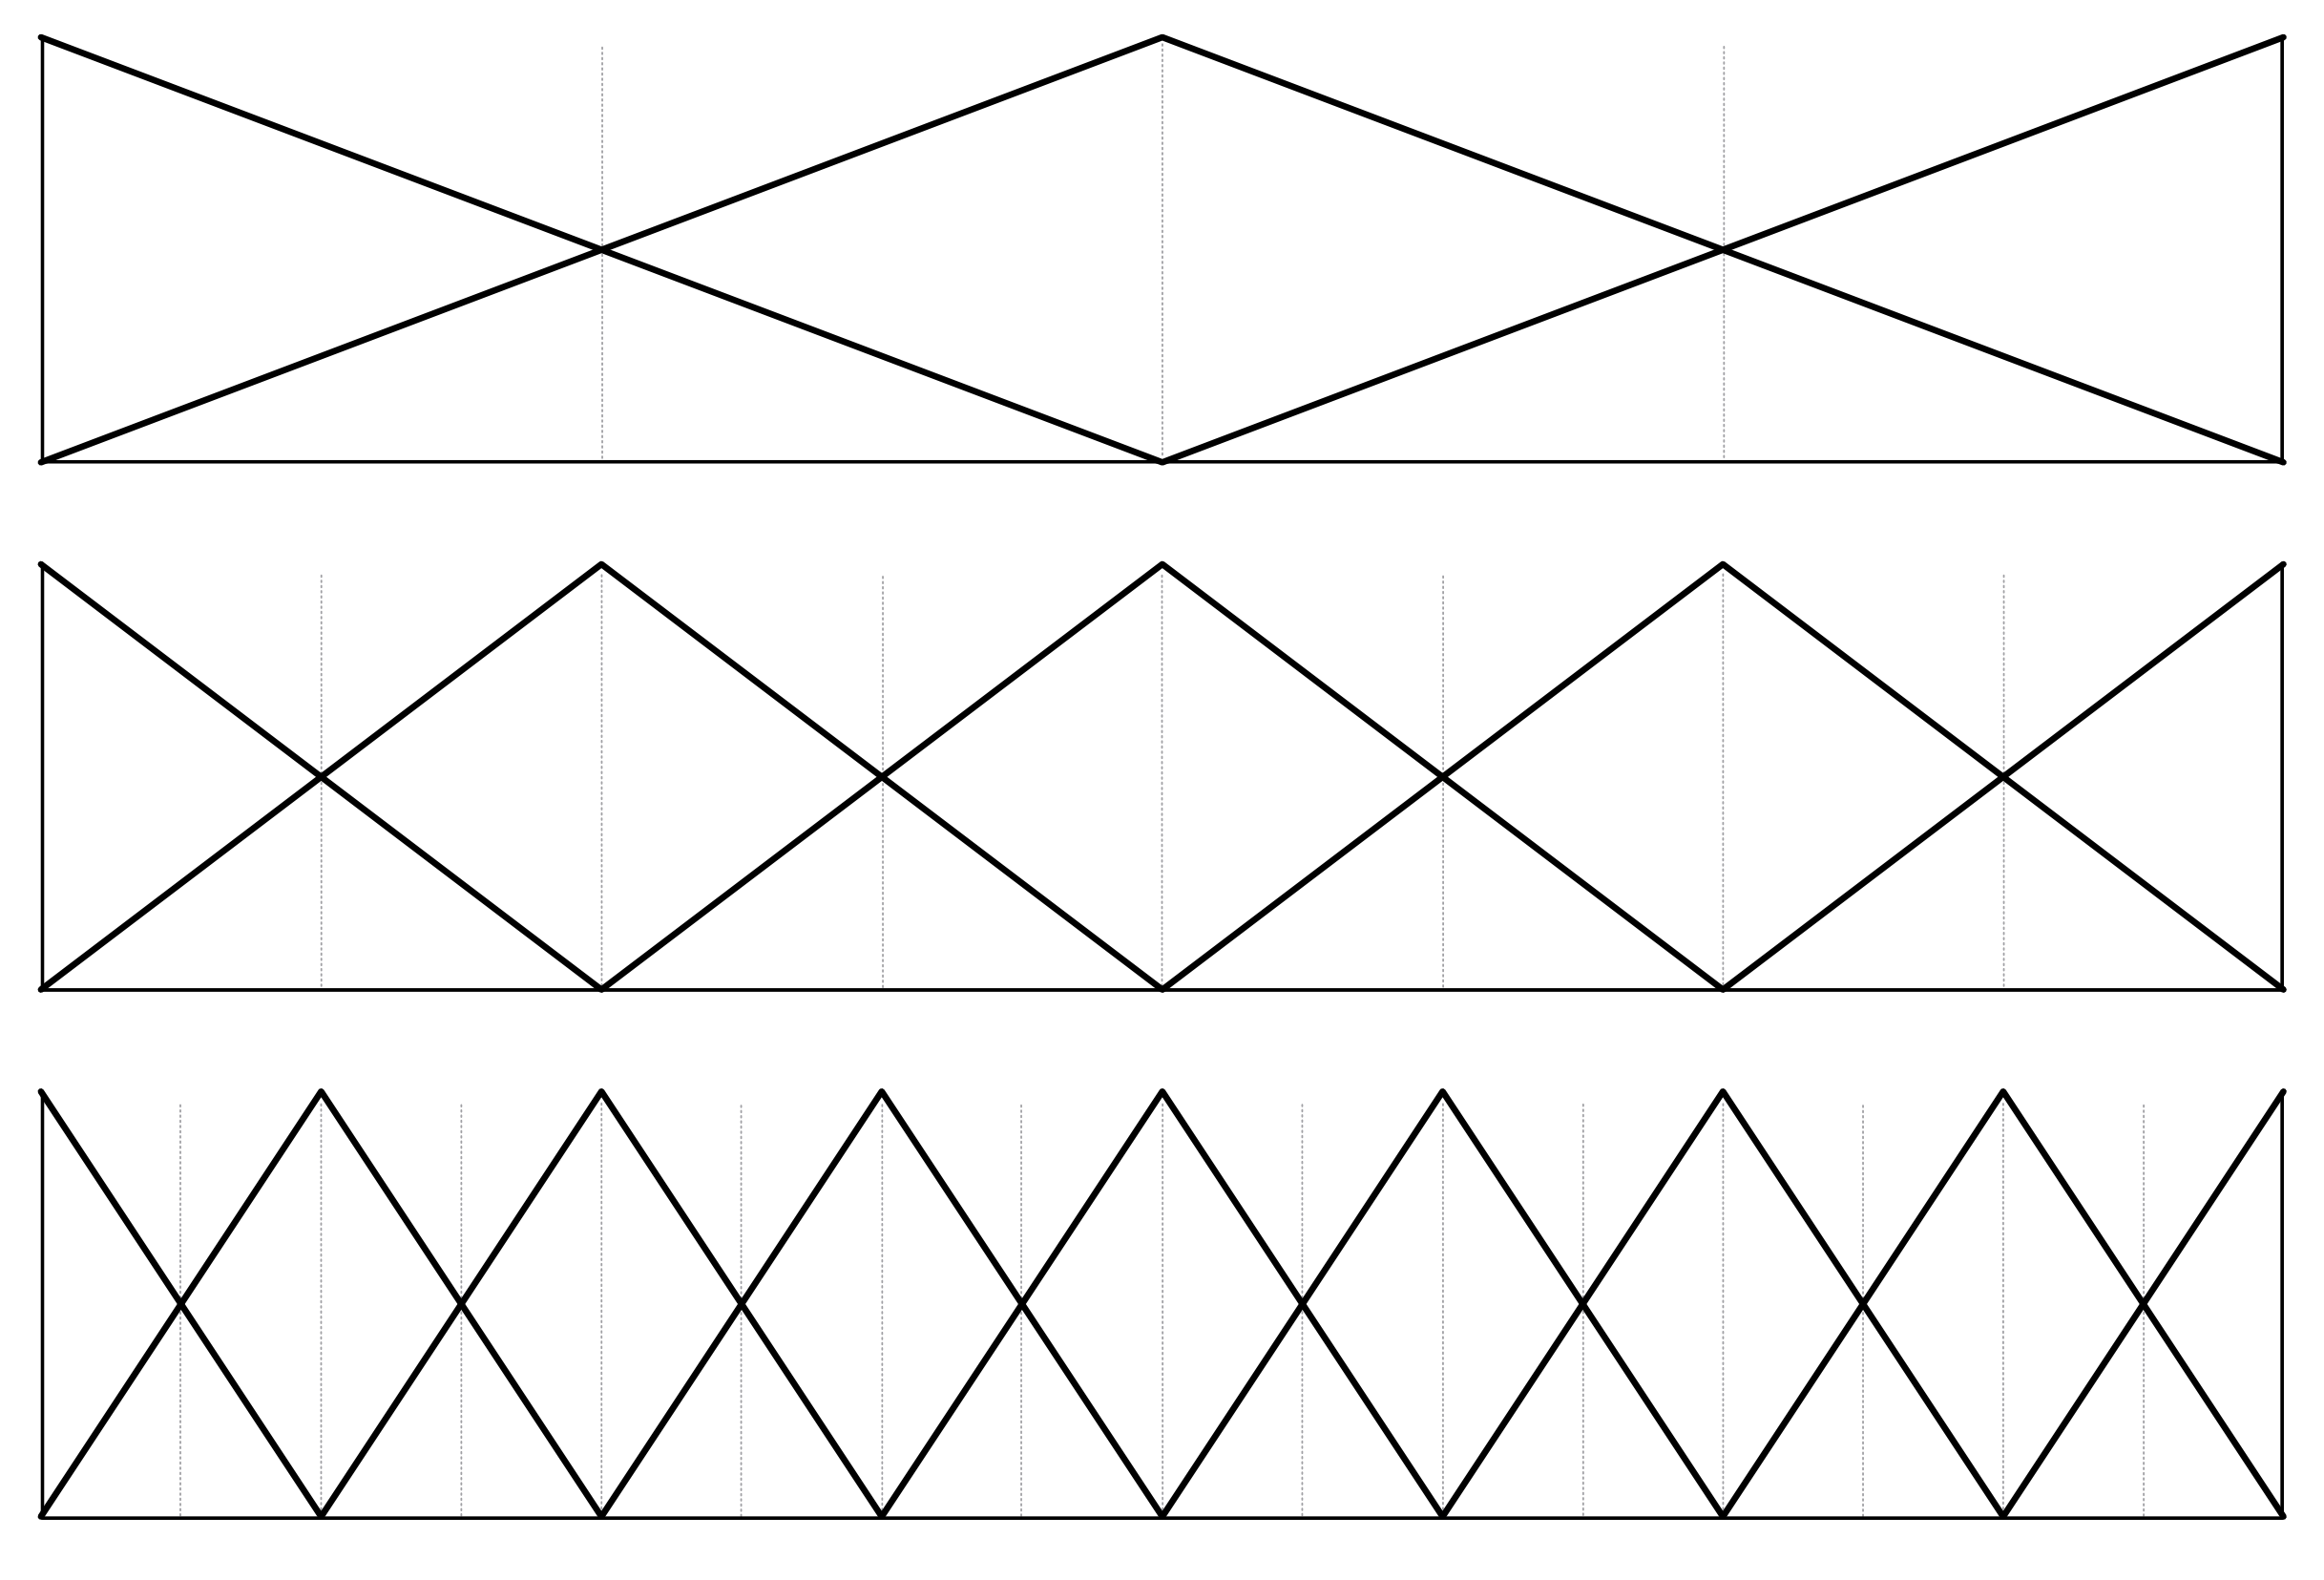
\includegraphics[width=\linewidth]
    {chapters/preferences/hierarchia_lingwistyczna}
  \caption{Przykładowa hierarchia lingwistyczna}
  \label{fig:hierarchia_lingwistyczna}
\end{figure}

W omawianym w tej pracy modelu podejmowania decyzji grupowej możliwe jest użycie
różnych zaprezentowanych powyżej sposobów wprowadzania preferencji. Z tego
powodu potrzebna jest transformacja z jednej metody na drugą. W przypadku
niesymetrycznej zmiennej lingwistycznej wygodne okazuje się przedstawienie jej
przy pomocy klasycznej zmiennej lingwistycznej. Najprostsza procedura wykonująca
tą czynność przy użyciu hierarchii lingwistycznej wygląda następująco:
\begin{enumerate}[i.]
  \item Znajdź poziom $t^-$ w $LH$ (ang. Linguistic Hierarchy) reprezentujący
  podzbiór termów $S^L_{UN}$ na lewo od środkowego termu w niesymetrycznym
  zbiorze termów lingwistycznych $S_{UN}$. Znaleziony poziom $LH$ powinien
  odpowiadać rozkładowi termów w $S^L_{UN}.$
  \item Znajdź poziom $t^+$ w $LH$ reprezentujący podzbiór termów $S^R_{UN}$ na
  prawo od środkowego termu ze zbioru $S_{UN}.$
  \item Środkowy term zbioru $S_{UN}$ przedstaw używając środkowych
  termów z poziomów $t^-$ i $t^+.$
\end{enumerate}

Okazuje się, że pojawia się problem, kiedy nie istnieje poziom $t^-$ lub $t^+$ w
$LH$ reprezentujący, odpowiednio, $S^L_{UN}$ lub $S^R_{UN}$. Dlatego Alonso et
al. zaprezentowali algorytm, który zakłada brak poziomu $t^-$, jak na rysunku
\ref{fig:niesymetryczna_zmienna} (przez analogię można napisać algorytm dla
$t^+$):
\begin{enumerate}[i.]
  \item Reprezentacja $S^L_{UN}\colon$
  \begin{enumerate}[(a)]
    \item Zidentyfikuj środkowy term $S^L_{mid}$ w $S^L_{UN}$.
    \item Znajdź poziom $t^-_2$ po lewej stronie zbiorów $LH^L$, który odpowiada
    lewemu podzbiorowi termów z $S^L_{UN}$, gdzie $LH^L$ oznacza lewą część
    $LH$.
    \item Znajdź poziom $t^+_2$ po prawej stronie zbiorów $LH^L$, który
    odpowiada prawemu podzbiorowi termów z $S^L_{UN}$.
    \item Przedstaw środkowy term $S^L_{mid}$ używając poziomów $t^-_2$ i
    $t^+_2$.
  \end{enumerate}
  \item Znajdź poziom $t^+$ w $LH$ reprezentujący podzbiór termów $S^R_{UN}$.
  \item Środkowy term zbioru $S_{UN}$ przedstaw używając środkowych termów z
  poziomów $t^+$ i $t^+_2$.
\end{enumerate}
\begin{figure}[ht]
  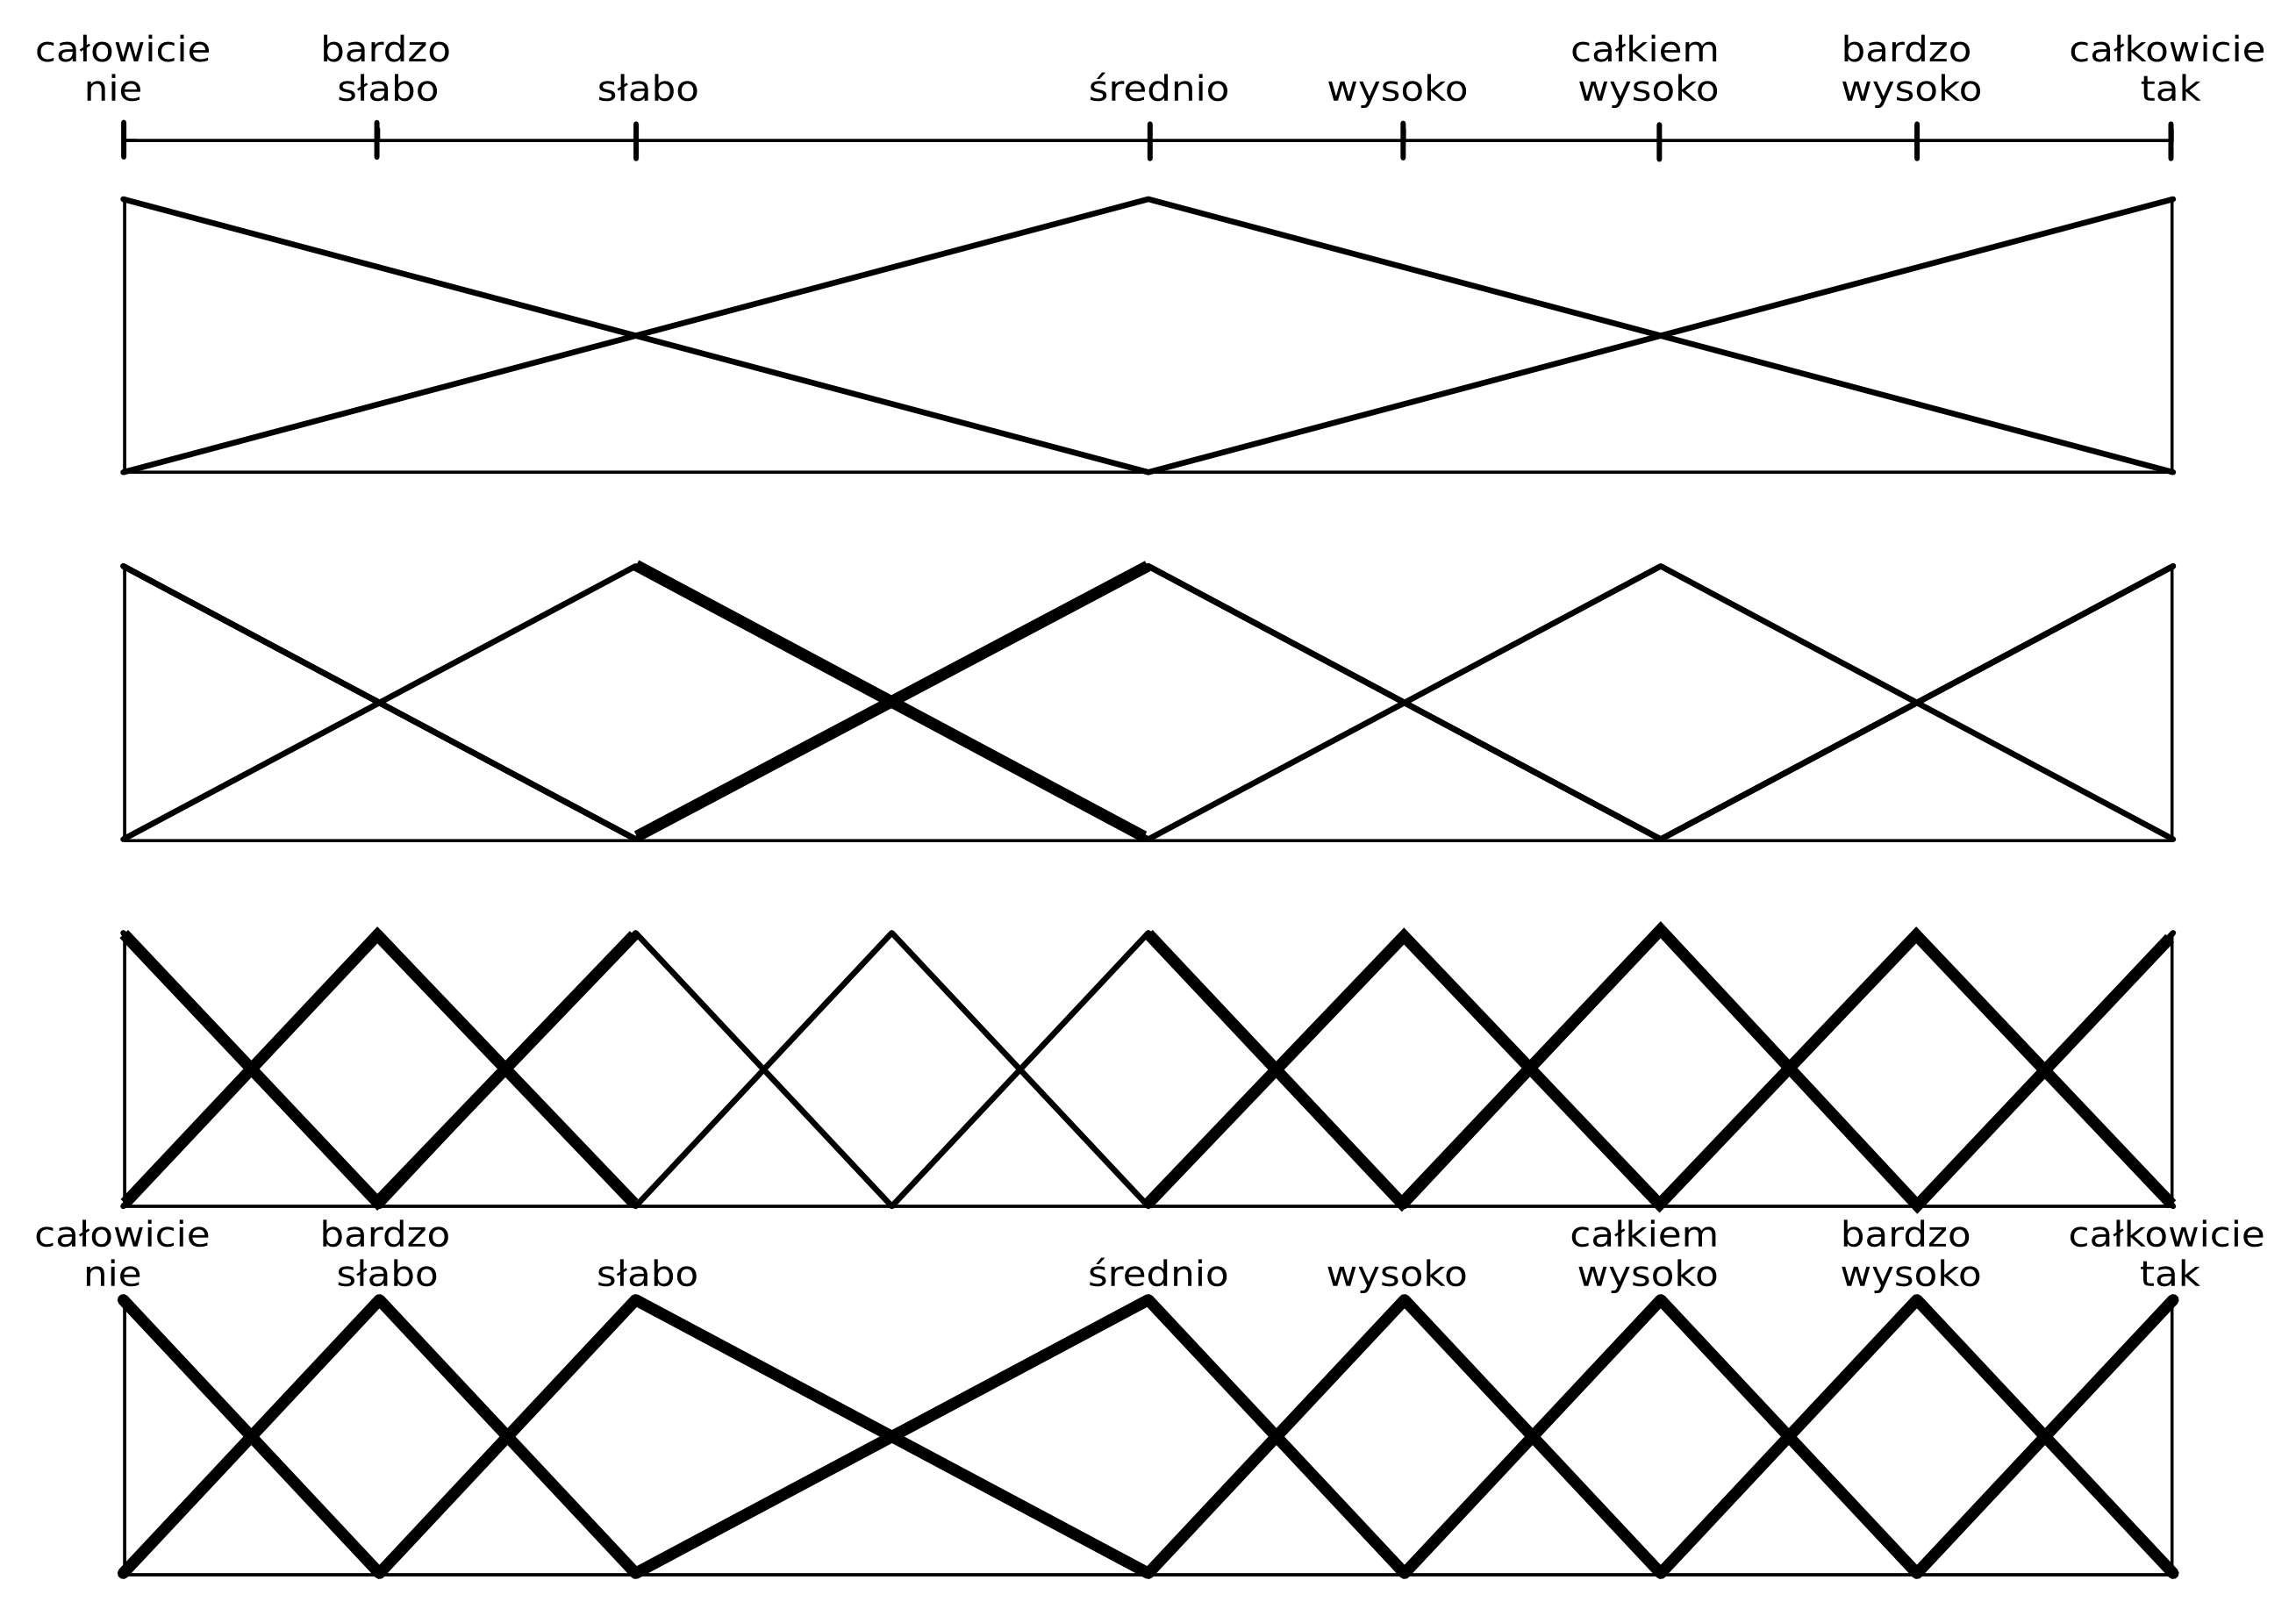
\includegraphics[width=\linewidth]
    {chapters/preferences/hierarchia_lingwistyczna_przyklad}
  \caption{Reprezentacja niesymetrycznej zmiennej lingwistycznej}
  \label{fig:hierarchia_lingwistyczna_przyklad}
\end{figure}
Przykład działania algorytmu został przedstawiony na rysunku
\ref{fig:hierarchia_lingwistyczna_przyklad}, na którym jest reprezentacja
niesymetrycznego zbioru termów lingwistycznych $S_{UN} = \{ N, VL, L,$ $M, H, 
QH, VH, T \}$ z rysunku \ref{fig:niesymetryczna_zmienna} dla hierarchii
lingwistycznej $LH$ z rysunku \ref{fig:hierarchia_lingwistyczna}.
W tym przykładzie mamy:
\begin{itemize}
  \item $S^L_{UN} = \{N,VL,L\},$
  \item $S^L_{mid} = L,$
  \item $LH^L = \{s_0^{n(1)}\} \cup \{s_0^{n(2)}, s_1^{n(2)}\} \cup
  \{s_1^{n(3)}, s_2^{n(3)}, s_3^{n(3)}\}.$
\end{itemize}
